\documentclass[11pt]{article}
\usepackage[a4paper,margin=1in]{geometry}
\usepackage{amsmath,amssymb,amsthm}
\usepackage{graphicx,float,microtype,booktabs,array,xcolor}
\usepackage[colorlinks=true,linkcolor=blue!55!black,urlcolor=blue!60!black]{hyperref}
\newtheorem{theorem}{Theorem}
\newtheorem{corollary}[theorem]{Corollary}
\newtheorem{remark}[theorem]{Remark}
\newcommand{\D}{\mathbb D}
\newcommand{\C}{\mathbb C}
\newcommand{\R}{\mathbb R}
\newcommand{\Hp}{H^p_+}
\newcommand{\Hq}{H^q_+}
\newcommand{\dist}{\operatorname{dist}}
\newcommand{\Kmin}{\mathcal K_{\min}}
\title{General-\(p\) Toeplitz Kernels:\\A Dual-Distance Criterion and a Minimal-Function Reduction}
\author{Automated mathematics run \texttt{fa\_banach\_001}\\Lane 0 --- candidate partial result}
\date{11 August 2026}
\begin{document}
\maketitle

\begin{center}
\fbox{\parbox{0.91\textwidth}{\textbf{Status.}
Substantial partial answer.  For every $1<p<\infty$ we give an exact
functional-analytic criterion for a Toeplitz kernel to consist only of bounded
functions.  We also prove that the minimal-function question has a positive
answer for every Toeplitz kernel possessing an exact outer-multiplier model-space
representation.  What remains is the structural, non-Hilbertian factorisation
problem needed to make that representation universal.}}
\end{center}

\section{The two source questions}

C\^amara--Malheiro--Partington first characterize those upper-half-plane model
spaces $K_\theta^p$ contained in $H^\infty_+$.  They then ask for a complete
answer for general Toeplitz kernels in $H^p_+$, outside the known Hilbert case.

\begin{figure}[H]
\centering
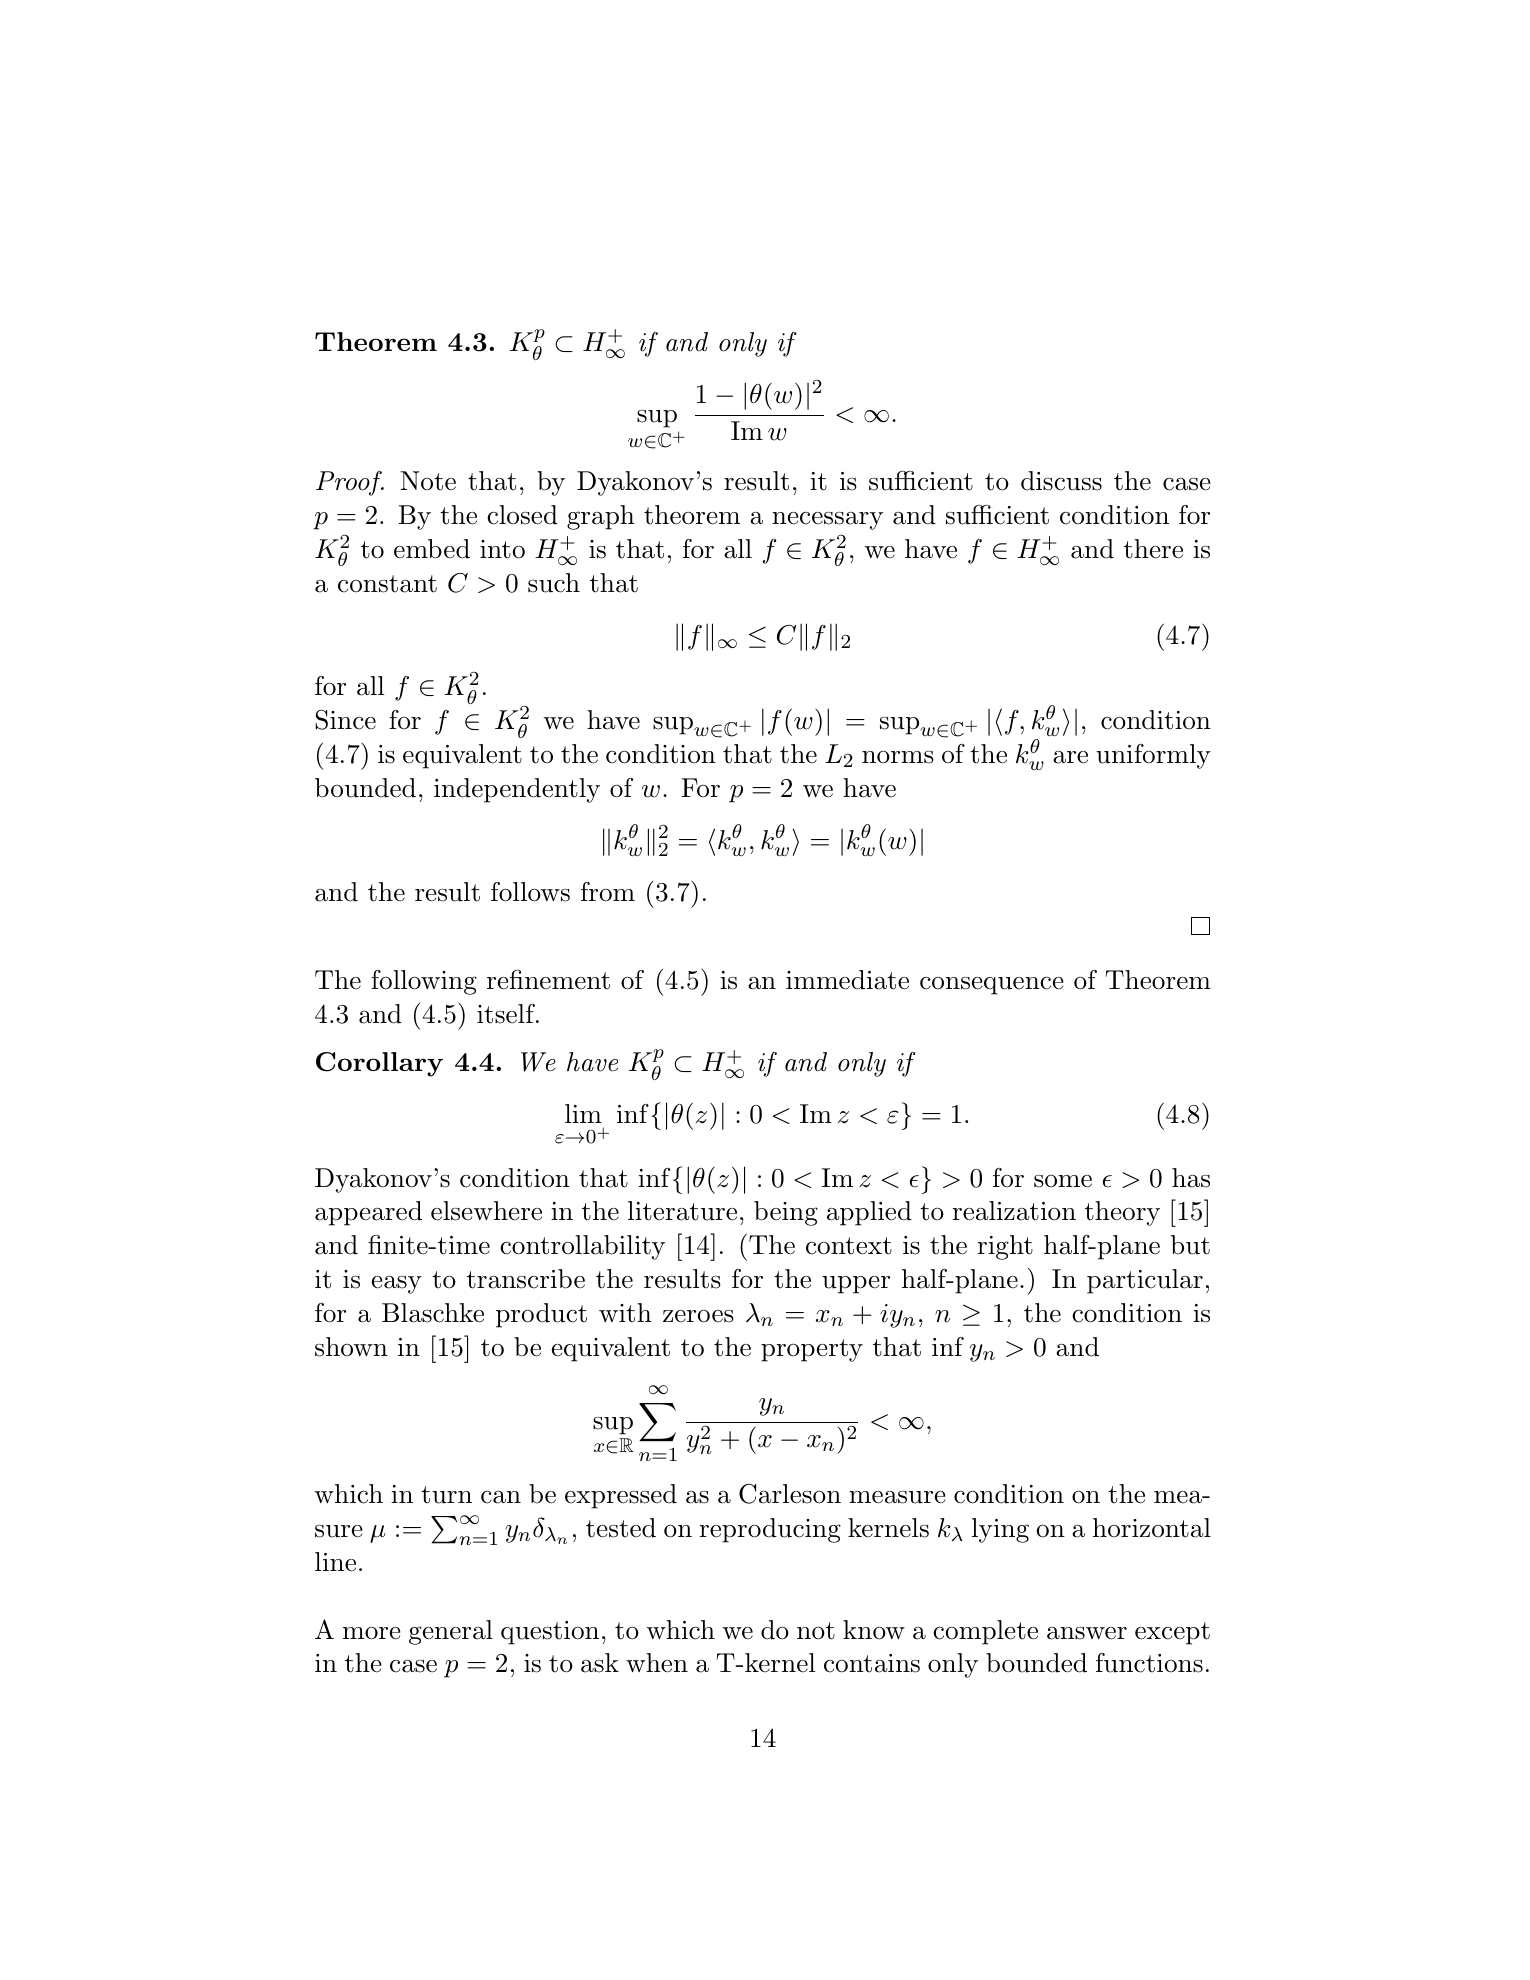
\includegraphics[width=0.84\textwidth,height=0.58\textheight,keepaspectratio]{figures/source_bounded_question-14.png}
\caption{Source PDF page 14: the general boundedness question.}
\end{figure}

The second question uses the following terminology.  If
$\mathcal K=\Kmin(IO)$ for an inner $I$ and outer $O$, then $O$ is a
\emph{minimal function} for $\mathcal K$ when
$\Kmin(O)=\operatorname{span}\{O\}$.  The source proves existence for all
model spaces and asks whether every nonzero proper Toeplitz kernel has such a
function.

\begin{figure}[H]
\centering
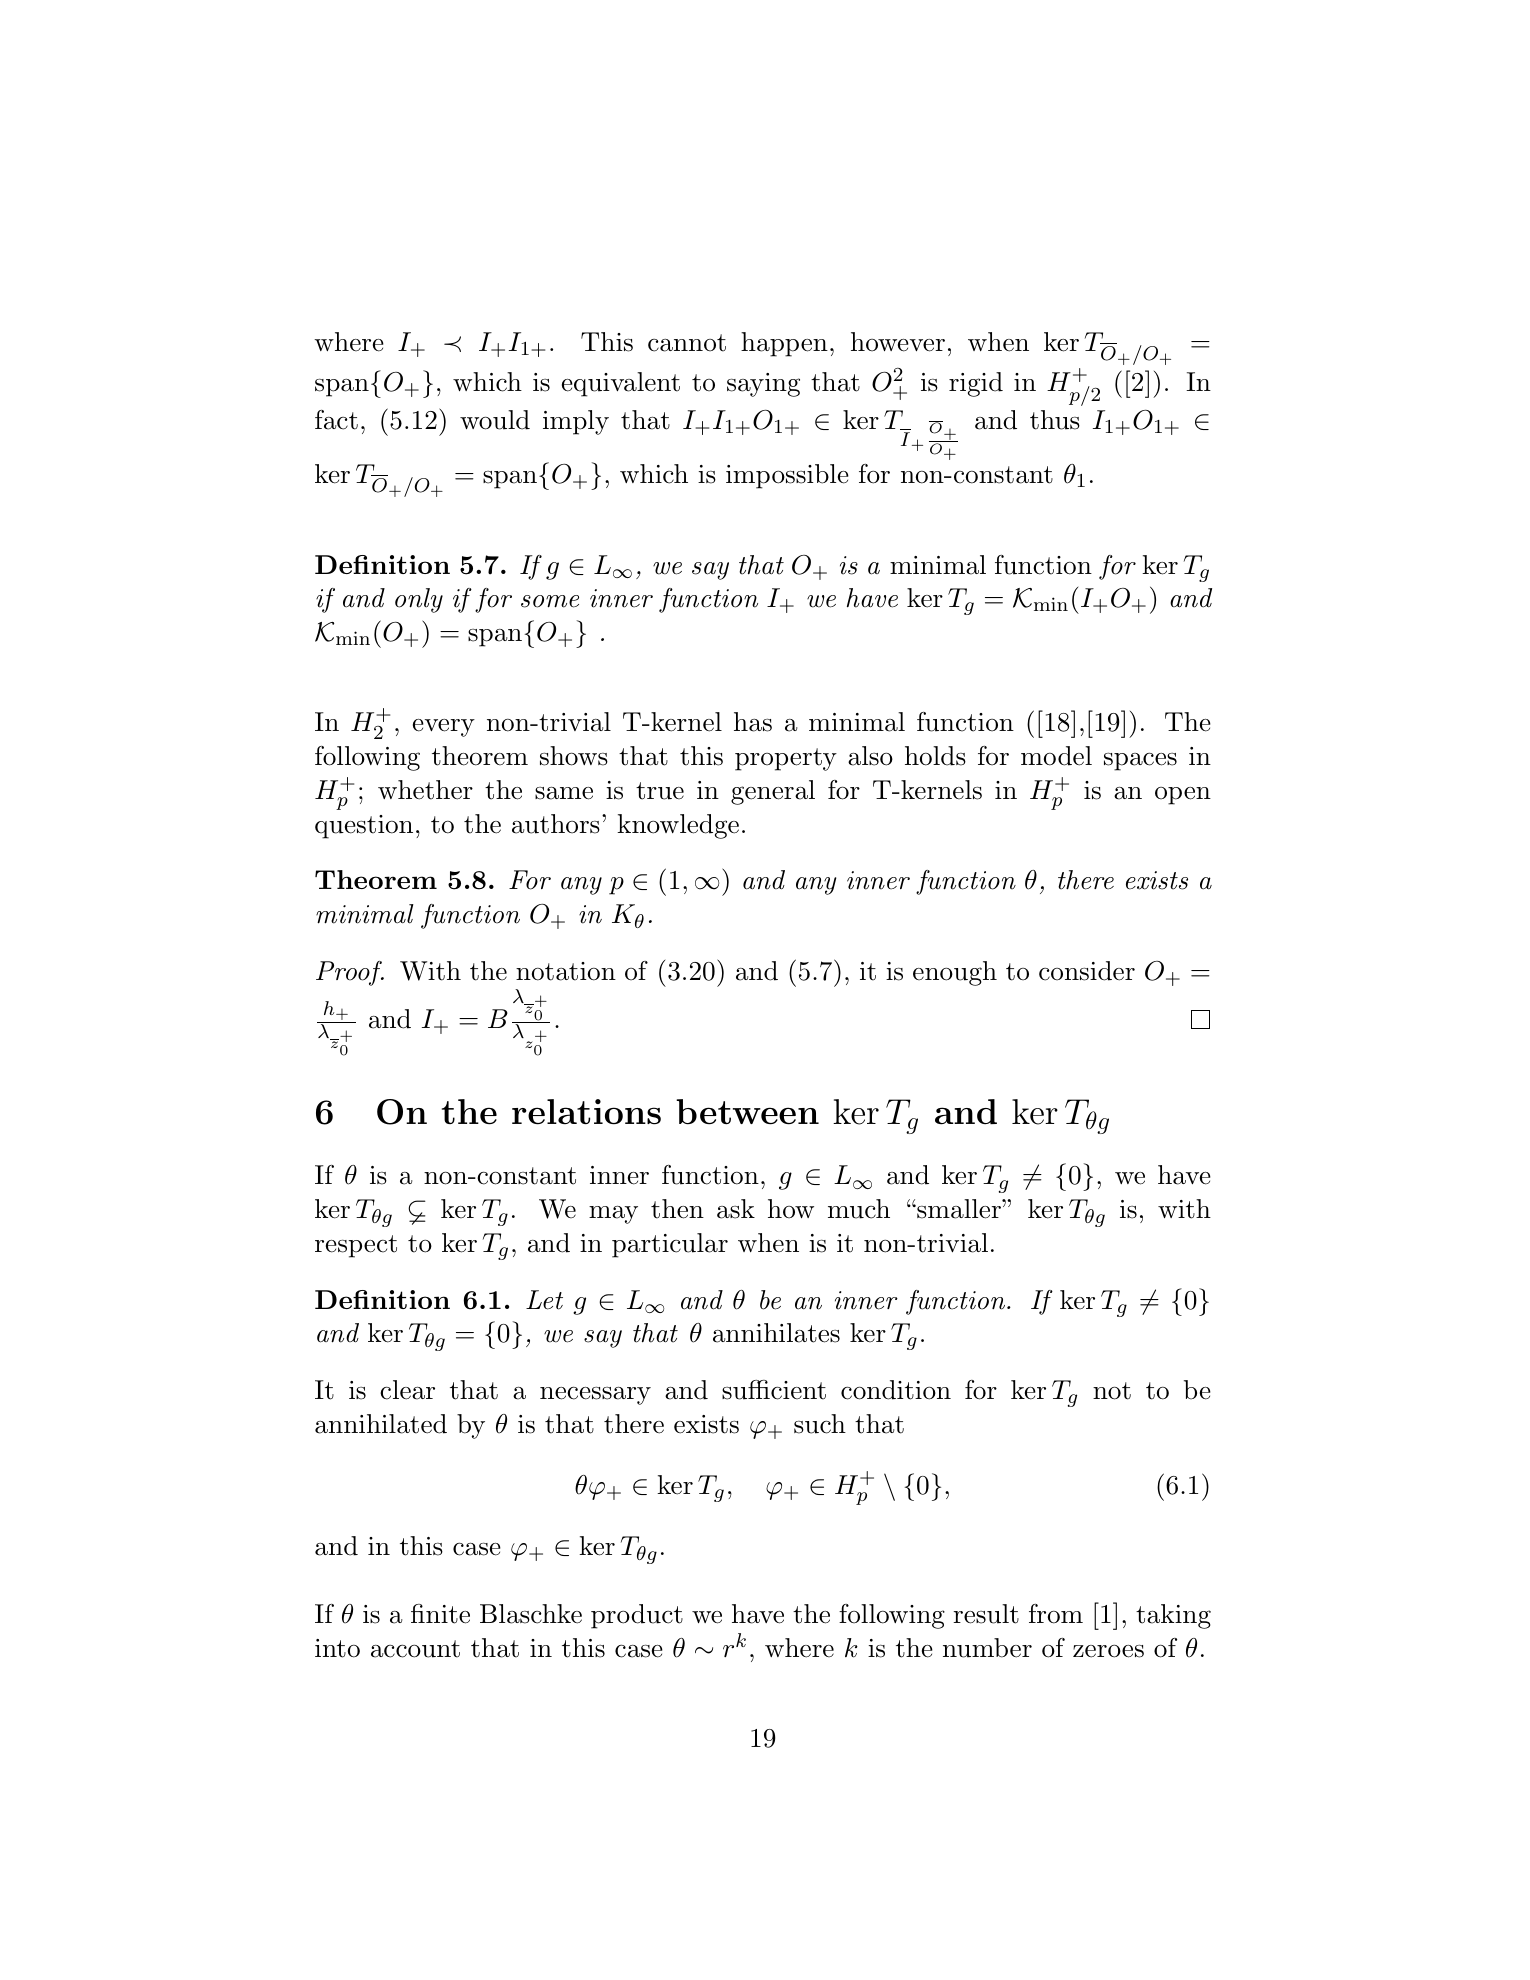
\includegraphics[width=0.84\textwidth,height=0.58\textheight,keepaspectratio]{figures/source_minimal_question-19.png}
\caption{Source PDF page 19: Definition 5.7 and the general minimal-function
question.}
\end{figure}

\section{An exact general-p boundedness criterion}

Work first on the upper half-plane, exactly as in the source.  Put
$q=p/(p-1)$ and use the duality
\[
 \langle f,h\rangle=\frac1{2\pi}\int_{\R}f(x)\overline{h(x)}\,dx
 \qquad(f\in H^p_+,\ h\in H^q_+).
\]
For $w\in\C_+$ let $k_w(x)=(x-\overline w)^{-1}$.  Cauchy's formula gives
$|f(w)|=|\langle f,k_w\rangle|$.  For $g\in L^\infty(\R)$ define
\[
 \mathcal R_g:=\overline{T_{\overline g}(H^q_+)}^{\,H^q_+}.
\]

\begin{theorem}[adjoint-range distance criterion]\label{thm:distance}
Let $1<p<\infty$, $g\in L^\infty(\R)$, and
$\mathcal K=\ker(T_g:H^p_+\to H^p_+)$.  Then
\[
 \mathcal K\subset H^\infty_+
 \quad\Longleftrightarrow\quad
 \sup_{w\in\C_+}\dist_{H^q_+}(k_w,\mathcal R_g)<\infty.                 \tag{2.1}
\]
In fact the supremum in \textup{(2.1)} is exactly the operator norm of the
inclusion $\mathcal K\hookrightarrow H^\infty_+$ under the normalization
above.  If the supremum is infinite, $\mathcal K$ contains an unbounded
function.
\end{theorem}

\begin{proof}
The adjoint of $T_g$ under $H^p_+$--$H^q_+$ duality is $T_{\overline g}$.
The annihilator identity for a bounded operator therefore gives
\[
 \mathcal K^\perp
   =(\ker T_g)^\perp
   =\overline{\operatorname{ran}T_g^*}
   =\mathcal R_g.
\]
By Hahn--Banach, restriction identifies $\mathcal K^*$ isometrically with
$H^q_+/\mathcal K^\perp$.  Hence
\[
 \|\operatorname{ev}_w|_{\mathcal K}\|
 =\|k_w+\mathcal K^\perp\|_{H^q_+/\mathcal K^\perp}
 =\dist_{H^q_+}(k_w,\mathcal R_g).                                    \tag{2.2}
\]
Taking the supremum first over $w$ and then over the unit ball of $\mathcal K$
shows that the right side of (2.1) is precisely the norm of the inclusion,
provided that inclusion is bounded.

It remains only to justify that set inclusion implies bounded inclusion.  If
$f_n\to f$ in $\mathcal K$ with the $H^p$ norm and $f_n\to F$ in the
$H^\infty$ norm, continuity of point evaluations in $H^p$ and locally uniform
convergence from $H^\infty$ give $f(w)=F(w)$ for every $w$.  Thus the graph is
closed, and the closed graph theorem applies.  The last assertion is the
contrapositive: if every member were bounded, the closed graph argument would
make the supremum finite.
\end{proof}

This is an exact answer in quotient geometry, valid without closed-range or
Fredholm hypotheses.  It is deliberately not advertised as the intrinsic
symbol-factorisation classification sought by the source: the closure
$\mathcal R_g$ can itself be difficult to compute.

\section{What an exact model-space representation buys}

For the second question it is cleaner to use the conformally equivalent disk
notation.  Let $K_\theta^p=\ker T_{\overline\theta}\subset H^p(\D)$ and
assume $\theta(0)=0$.  Recall that
\[
 \Kmin(f)=\ker T_{\overline z\,\overline I\,\overline O/O}
 \quad\text{when } f=IO
\]
is the inner--outer factorization of $f$.  The standard Cayley isometry gives
the corresponding upper-half-plane statement.

\begin{theorem}[outer model multipliers are minimal functions]\label{thm:model}
Let $1<p<\infty$.  Suppose a nonzero proper Toeplitz kernel
$\mathcal K\subset H^p(\D)$ has an exact representation
\[
 \mathcal K=wK_\theta^p,                                               \tag{3.1}
\]
where $\theta$ is inner with $\theta(0)=0$ and $w$ is outer.  Then
\[
 \Kmin(w)=\operatorname{span}\{w\},                                   \tag{3.2}
\]
$w\theta/z$ is a maximal function for $\mathcal K$, and therefore $w$ is a
minimal function for $\mathcal K$ in the sense of the source.
\end{theorem}

\begin{proof}
Since $1\in K_\theta^p$, (3.1) gives $w\in\mathcal K$.  Minimality of
$\Kmin(w)$ among Toeplitz kernels containing $w$ gives
$\Kmin(w)\subset\mathcal K$.  If $f\in\Kmin(w)$, write $f=wk$ with
$k\in K_\theta^p\subset H^p$.  On the other hand,
$f\in\ker T_{\overline z\,\overline w/w}$ implies
\[
 \frac f w=\frac{\overline h}{\overline w}
 \quad\text{for some }h\in H^p.
\]
Thus $f/w$ belongs both to $H^p\subset\mathcal N^+$ and to
$\overline{\mathcal N^+}$.  The Smirnov intersection theorem makes it
constant.  This proves (3.2).

Now $\theta/z$ is inner and is a maximal function for $K_\theta^p$.  Let
$m=w\theta/z$ and suppose $m\in\ker T_a$ for a bounded symbol $a$.  Every
$k\in K_\theta^p$ can be written
$k=(\theta/z)\overline n$ with $n\in\mathcal N^+$ and with the displayed
product in $H^p$.  Hence every $f=wk\in\mathcal K$ has the form
$f=m\overline n$.  Since $am\in\overline{H_0^p}$ and
$af\in L^p\cap\overline{\mathcal N^+}$, the Smirnov theorem gives
$af\in\overline{H_0^p}$.  Therefore
$\mathcal K\subset\ker T_a$, proving $\Kmin(m)=\mathcal K$.  The
inner--outer factors of $m$ are $\theta/z$ and $w$, and (3.2) is exactly the
remaining clause in the definition of a minimal function.
\end{proof}

\begin{corollary}[boundedness inside the same class]
Under (3.1), put $q=p/(p-1)$ and
$k_\lambda(z)=(1-\overline\lambda z)^{-1}$.  Then
\[
 \mathcal K\subset H^\infty
 \quad\Longleftrightarrow\quad
 \sup_{\lambda\in\D}|w(\lambda)|
 \dist_{H^q}(k_\lambda,\theta H^q)<\infty.                             \tag{3.3}
\]
For $p=2$, the distance in (3.3) is
$\sqrt{(1-|\theta(\lambda)|^2)/(1-|\lambda|^2)}$.
\end{corollary}

\begin{proof}
Apply Theorem~\ref{thm:distance}, in disk form, to $K_\theta^p$ and then to
the evaluation of $wk$.  Since
$(K_\theta^p)^\perp=\theta H^q$, the norm of evaluation at $\lambda$ on
$K_\theta^p$ is the displayed distance.  Multiplication by $w$ multiplies
that evaluation functional by $w(\lambda)$.  The $p=2$ formula is the norm of
the usual model-space reproducing kernel.
\end{proof}

\section{Why the result remains partial}

In $H^2$, Hayashi's theorem represents every nontrivial Toeplitz kernel as
$wK_\theta^2$ with an outer isometric multiplier $w$; Theorem~\ref{thm:model}
then recovers the positive Hilbert answer.  Away from $p=2$, the strongest
general representation found in the literature is the extremal/intersection
form recorded by O'Loughlin (reformulating Hartmann--Seip): for an extremal
$q_0$ and inner $I$,
\[
 \ker T_g=q_0K_I^p\cap H^p\quad(p\le2),\qquad
 \ker T_g=q_0K_I^2\cap H^p\quad(p\ge2).                                \tag{4.1}
\]
The intersection in (4.1) cannot be removed unless multiplication by $q_0$
maps the entire indicated model space into $H^p$.  That missing onto-divisor
property is precisely what is automatic in the Hilbert case and what would
turn Theorem~\ref{thm:model} into a full answer.

Six focused upgrade attempts were made: adjoint-range duality, closed-range
factorisation, extremal-vector rigidity, exact model multipliers, removal of
the intersection in (4.1), and transfer across $p=2$.  The last route fails in
opposite directions: for $p>2$ a Hilbert minimal factor need not lie in $H^p$,
while for $p<2$ rigidity in $H^1$ need not imply rigidity in the larger
$H^{p/2}$ class.  The packet therefore stops at the strongest proved claims
rather than assuming the non-Hilbert divisor theorem it would need.

\section{Novelty and verification}

The two proofs above are self-contained apart from standard Hardy-space
duality, the Smirnov intersection theorem, and the source's minimal-kernel
formula.  Searches through the exact phrases, later arXiv literature, and the
run indexes did not locate these two statements verbatim.  The distance
criterion is an elementary Banach-duality consequence and should be treated as
a useful reformulation unless expert review establishes novelty.  The
model-multiplier theorem is the mathematically stronger partial advance.

\begin{thebibliography}{9}
\bibitem{CMP} M.~C.~C\^amara, M.~T.~Malheiro, and J.~R.~Partington,
\emph{Model spaces and Toeplitz kernels in reflexive Hardy spaces}, Oper.
Matrices 10 (2016), 127--148,
\href{https://arxiv.org/abs/1507.05797}{arXiv:1507.05797}.
\bibitem{OL} R.~O'Loughlin, \emph{Toeplitz kernels and the backward shift},
J. Math. Anal. Appl. 492 (2020), 124489,
\href{https://arxiv.org/abs/2001.10890}{arXiv:2001.10890}.
\bibitem{Unbounded} M.~C.~C\^amara, M.~T.~Malheiro, and J.~R.~Partington,
\emph{Kernels of unbounded Toeplitz operators and factorization of symbols},
Results Math. 76 (2021), article 28,
\href{https://arxiv.org/abs/2004.09985}{arXiv:2004.09985}.
\bibitem{CCD} M.~C.~C\^amara, C.~Carteiro, and C.~Diogo,
\emph{Maximal functions, conjugations and multipliers between Toeplitz
kernels}, \href{https://arxiv.org/abs/2512.20406}{arXiv:2512.20406}.
\end{thebibliography}
\end{document}
